\section{Theorie}


\begin{flushleft}
    Licht besteht aus elektromagnetischen Wellen und ist somit durch die Maxwell Gleichungen beschreibbar.
    Licht, welches im sichtbaren Bereich liegt, hat eine Wellenlänge zwischen $380\unit{\nano\meter}$ und $780\unit{\nano\meter}$.
    Das Ultraviolette Spektrum liegt unter den $380\unit{\nano\meter}$ bzw. zwischen $100\unit{\nano\meter}$ und $380\unit{\nano\meter}$, wobei das Infrarotspektrum über den $780\unit{\nano\meter}$ liegt, genauer gesagt zwischen $780\unit{\nano\meter}$ und $1\unit{\milli\meter}$
\end{flushleft}

\subsection{Strahlenoptik}

\begin{align}
    \intertext{Die Wellennormale beschreibt in der Strahlenoptik die Ausbreitung der Welle.
    Dabei ist die Ausbreitungsgeschwindigkeit unterschiedlich groß, welches von dem Material abhängt.
    Beim Auftreffen eines Lichtstrahles auf die Grenzfläche eines Mediums wird der Lichtstrahl gebrochen.
    Dabei entstehen zwei Ausbreitungsgeschwindigkeiten, $\text{v}_{1}$ und $\text{v}_{2}$, die durch die beiden Brechungsindizes der Medien, $\text{n}_{1}$ und $\text{n}_{2}$, sowie durch den Einfallswinkel $\alpha$ und Brechungswinkel $\beta$ beschrieben werden können  }
    \frac{\sin(\alpha)}{\sin(\beta)} = \frac{\text{v}_{1}}{\text{v}_{2}} = \frac{\text{n}_{2}}{\text{n}_{1}}\,. \label{1}
    \intertext{Luft ist ebenfalls ein Medium, dessen Ausbreitungsgeschwindigkeit bei $ \text{v}_{1} = 2,9979 \cdot 10^{8} \frac{\unit{\meter}}{\unit{\second}} $ liegt und einen Brechungsindex von $\text{n}_{1} = 1,000292$ besitzt.
    Das Medium,in welchen die Ausbreitungsgeschwindigkeit des Lichts größer ist als in dem anderen Medium, gilt als optisch dichteres Medium.
    Dadurch gilt, dass bei geringerer Ausbreitungsgeschwindigkeit von einem optisch dünneren Medium gesprochen wird.  }
\end{align}

\subsection{Reflexion} 

\begin{align}
    \intertext{Das Reflexionsgesetz besagt, dass wenn ein Lichtstrahl auf eine Grenzfläche auftrifft und reflektiert wird, ist der Einfallswinkel gleich dem Ausfallswinkel }
    \alpha_{1} = \alpha_{2}\,. \label{2}
\end{align}

\begin{figure}[H]
    \centering
    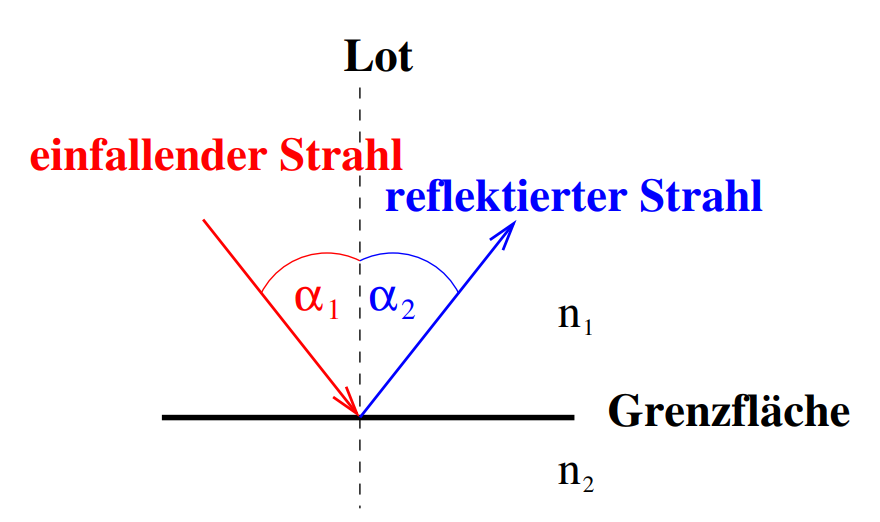
\includegraphics[height=40mm]{bilder/Ab1.png}
    \caption{Das reflektieren eines Lichtstrahles \cite{a1}.\label{Abbildung1} }
\end{figure}


\subsection{Brechung} 

\begin{align}
    \intertext{Brechung des Lichtes wird mit dem Snellius Gesetz erklärt, welches besagt, dass beim Auftreffen eines Lichtstrahl auf ein anderes Medium mit einem Brechungsindex n, dieser gebrochen wird.
    Dadurch wird der Ausfallswinkel als $\beta$ beschrieben}
    \text{n}_{1} \sin(\alpha) = \text{n}_{2} \sin(\beta)\,.\label{3}
\end{align}

\begin{figure}[H]
    \centering
    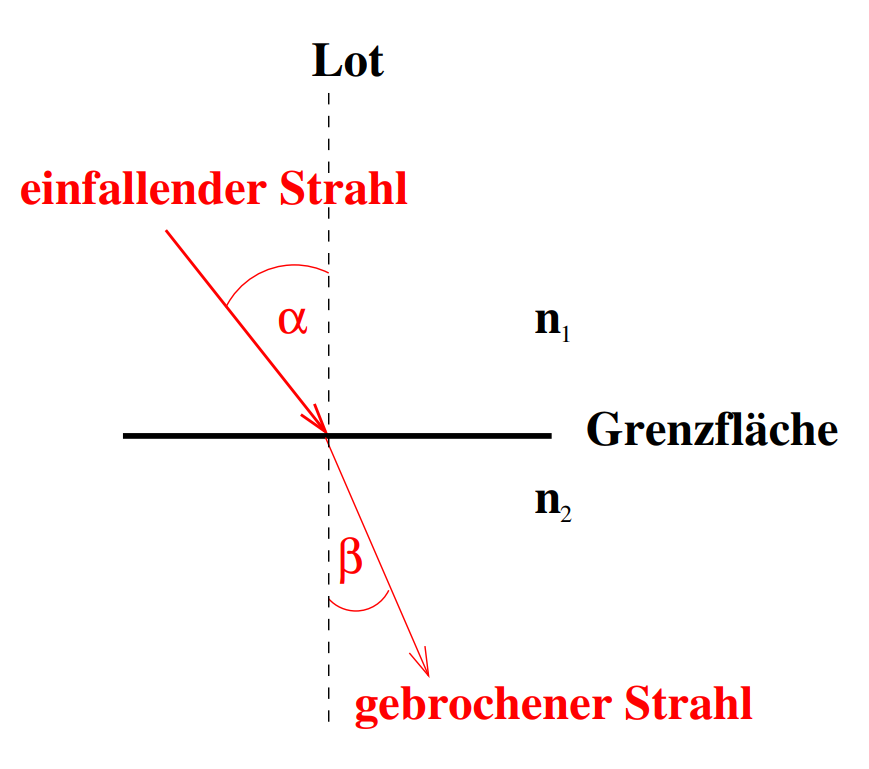
\includegraphics[height=45mm]{bilder/Ab2.png}
    \caption{Das brechen eines Lichtstrahles \cite{a1}. \label{Abbildung2} }
\end{figure}

\subsection{Reflexion und Transmission}

\begin{align}
    \intertext{Oft wird Licht nicht vollständig reflektiert, wenn es auf die Grenzfläche eines Mediums trifft.
    Der Teil des Lichtstrahles, der nicht reflektiert wird, wird transmittiert bzw. gebrochen.
    Dabei gilt das der Teil der reflektiert wird und der Teil der gebrochen wird, zusammen 1 ergibt}
    \text{R} + \text{T} = 1\,. \notag
\end{align}

\begin{figure}[H]
    \centering
    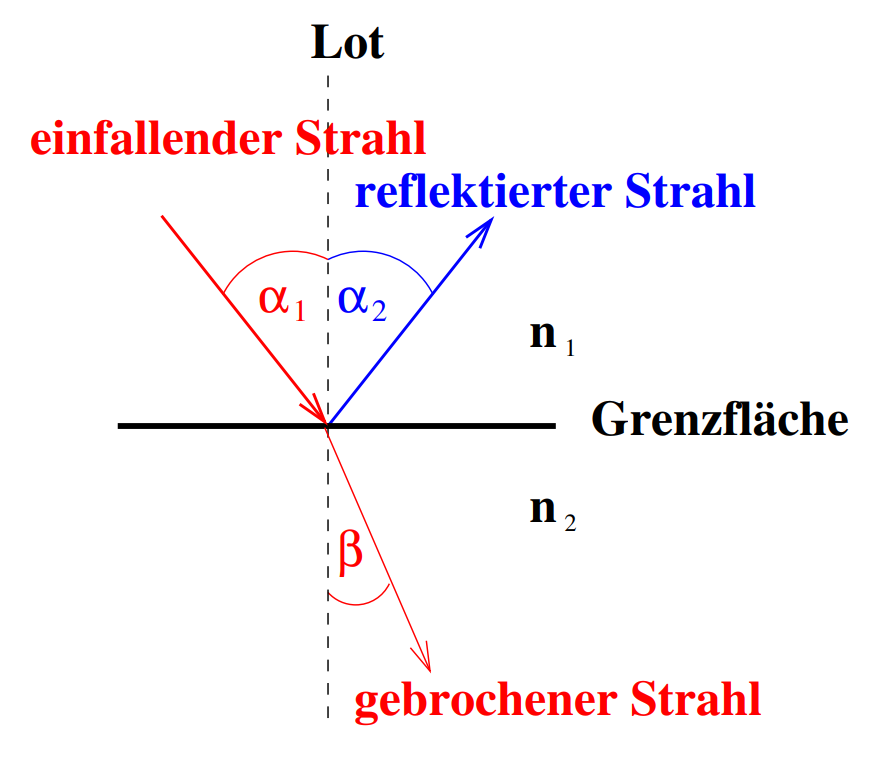
\includegraphics[height=45mm]{bilder/Ab3.png}
    \caption{Das reflektieren und brechen eines Lichtstrahles \cite{a1}. \label{Abbildung3} }
\end{figure}

\subsection{Wellenoptik}

\begin{flushleft}
    Beim Auftreffen des Lichtes auf ein Objekt, welches im Verhältnis zur Wellenlänge klein ist, breitet sich dieses auch im Schattenraum aus, da die geometrische Optik dafür nicht mehr ausreicht.
    Dabei sind Frequenz f, Wellenlänge $\lambda$ und Ausbreitungsgeschwindigkeit v, charakteristische Merkmale einer Welle, dessen Wellenzüge nicht länger als $10^{-8}\,\unit{\second}$ dauern.
    Durch eine Superpostion der Wellen können dennoch Interferenzbilder entstehen, wobei unter konstruktiver und destruktiver Interferenz unterschieden wird. 
    Beträgt der Gangunterschied bei gleicher Intensität $\lambda/2$, führt dies zu einer vollständigen Auslöschung der Welle.
\end{flushleft}

\subsection{Beugung am Gitter}

\begin{align}
    \intertext{Liegt bei der Ausbreiten der Lichtwelle ein Hindernis auf dem Weg, welches im Vergleich zur Wellenlänge klein ist, so kann es zu einer Beugung führen.
    Das Huygensche Prinzip beschreibt diese Ausbreitung und besagt, dass jeder Punkt auf einer Wellenfront eine neue Elementarwelle, welche die gleiche Frequenz hat, erzeugt.
    Befindet sich nun ein Spalt im Abstand L mit einem Schirm dahinter, wird ein Interferenzmuster beobachtbar. 
    Die dabei entstehenden Interferenzmaxima ergeben sich durch   }
    \text{a}\,\,\sin(\alpha) = \text{k}\,\lambda \,, \label{4}
    \intertext{wobei a die Spaltbreite, k das k-te Intensitätsminimum und $\lambda$ die Wellenlänge darstellt.
    Diese Intensitätsminima befindet sich in einem Winkel von $\alpha$ relativ zur geradlinigen Ausbreitungsrichtung.
    Dieses Prinzip lässt sich auf ein Strichgitter mit n-Einfachspalten gleicher Breite, mit der Gitterkonstante d, übernehmen.
    Dadurch ergibt sich für die Interferenzmaxima k-ter Ordnung die Beziehung }
    \text{d}\,\,\sin(\alpha) = \text{k}\,\lambda\,. \label{5}
\end{align}